\section*{Exercises 7.3}
%
\begin{enumerate}
\xitem Let  $A = \left\{ {a, b, c, d, e} \right\}$  and let  $\sim$  be the relation on   $A$  that is represented by the directed graph in Figure~\ref{fig:dirgraph-exer1}.
\label{exer:sec73-1}%

\begin{figure}[h]
\begin{center}
\scalebox{0.8}{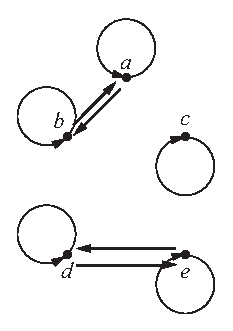
\includegraphics{figps-exer73digraph.eps}}
\caption{Directed Graph for the Relation in Exercise~(\ref{exer:sec73-1})}
\label{fig:dirgraph-exer1}%
\end{center}
\end{figure}

Prove that  $\sim$  is an equivalence relation on the set  $A$, and determine all of the equivalence classes determined by this equivalence relation.

\xitem  Let $A = \left\{ a, b, c, d, e, f \right\}$, and assume that $\sim$ is an equivalence relation on $A$.  Also assume that it is known that
\label{exer:drawdirgraph}%
$$
\BeginTable
\BeginFormat
| p(1in) | p(1in) | p(1in) |
\EndFormat
" $a \sim b$  "  $a \not \sim c$  "  $e \sim f$ " \\
" $a \sim d$  "  $a \not \sim f$  "  $e \not \sim c$. " \\
\EndTable
$$
%\begin{center}
%\begin{multicols}{3}
%$a \sim b$
%
%$a \sim d$
%
%$a \not \sim c$
%
%$a \not \sim f$
%
%$e \sim f$
%
%$e \not \sim c$
%\end{multicols}
%\end{center}
\noindent
Draw a complete directed graph for the equivalence relation  $\sim$  on the set $A$, and then determine all of the equivalence classes for this equivalence relation.

\xitem Let   $A = \left\{ {0, 1, 2, 3,  \ldots , 999, 1000} \right\}$.  Define the relation  $R$  on  $A$  as follows: \label{exer:sec73-2}

\begin{list}{}
\item For  $x, y \in A$,  $x \mathrel{R} y$ if and only if  $x$  and  $y$  have the same number of digits.
\end{list}

\noindent
Prove that  $R$  is an equivalence relation on the set  $A$  and determine all of the distinct equivalence classes determined by  $R$.

\item Determine all of the congruence classes for the relation of congruence modulo  5  on the set of integers. \label{exer:sec73-congclass}

\item Let $\Z_{9} = \left\{ 0, 1, 2, 3, 4, 5, 6, 7, 8 \right\}$.  \label{exer:modpowers}
\begin{enumerate}
\yitem Define the relation $\sim$ on $\Z_{9}$ as follows:  For all $a, b \in \Z_{9}$, $a \sim b$ if and only if $a^2 \equiv b^2 \pmod {9}$.  Prove that $\sim$ is an equivalence relation on 
$\Z_{9}$ and determine all of the distinct equivalence classes of this equivalence relation.

\item Define the relation $\approx$ on $\Z_{9}$ as follows:  For all $a, b \in \Z_{9}$, 
$a \approx b$ if and only if $a^3 \equiv b^3 \pmod {9}$.  Prove that $\approx$ is an equivalence relation on $\Z_{9}$ and determine all of the distinct equivalence classes of this equivalence relation.
\end{enumerate}

\item \label{exer:sec73-integer} Define the relation $\sim$ on $\Q$ as follows:  For $a, b \in \Q$, $a \sim b$ if and only if $a - b \in \Z$. \label{exer:sec72-integer}  In Progress Check~\ref{prog:example-equiv} of Section~\ref{S:equivrelations}, we showed that the relation $\sim$ is an equivalence relation on $\Q$.  Also, see Exercise~(\ref{exer:sec72-diffQ}) in Section~\ref{S:equivrelations}.

\begin{enumerate}
\yitem Prove that $\left[ \dfrac{5}{7} \right] = \left\{ \left. m + \dfrac{5}{7} \right| m \in \Z \right\}$.

\item If $a \in \Z$, then what is the equivalence class of $a$?

\item If $a \in \Z$, prove that there is a bijection from $\left[ a \right]$ to 
$\left[ \dfrac{5}{7} \right]$. 
\end{enumerate}

\item Define the relation $\sim$ on $\R$ as follows:
\label{exer:sec73-rationaldiff}%

\begin{center}
For $x, y \in \R$, $x \sim y$ if and only if $x - y \in \Q$.
\end{center}

\begin{enumerate}
\item Prove that $\sim$ is an equivalence relation on $\R$.
\item List four different real numbers that are in the equivalence class of $\sqrt{2}$.
\item If $a \in \Q$, what is the equivalence class of $a$?
\item Prove that $\left[ \sqrt{2} \right] = \left\{ r + \sqrt{2} \mid r \in \Q \right\}$.
\item If $a \in \Q$, prove that there is a bijection from $\left[ a \right]$ to 
$\left[ \sqrt{2} \right]$.
\end{enumerate}


\item Define the relation $\sim$ on $\Z$ as follows:  For $a, b \in \Z$, $a \sim b$ if and only if $2a + 3b \equiv 0 \pmod 5$.  The relation $\sim$ is an equivalence relation on 
$\Z$.  (See Exercise~(\ref{exer:modequivrel}) in Section~\ref{S:equivrelations}).  Determine all the distinct equivalence classes for this equivalence relation.


\item Let  $A = \mathbb{Z} \times \left( {\mathbb{Z} - \left\{ 0 \right\}} \right)$.  That is,  $A = \left\{ { {\left( {a, b} \right) \in \mathbb{Z} \times \mathbb{Z} } \mid b \ne 0} \right\}$.  Define the relation  $ \approx $ on  $A$  as follows: \label{exer:sec73-rationals}

\begin{list}{}
\item For  $\left( {a, b} \right), \left( {c, d} \right) \in A$,  
$\left( {a, b} \right) \approx \left( {c, d} \right)$ if and only if  $ad = bc$.
\end{list}

\begin{enumerate}
  \yitem Prove that  $ \approx $  is an equivalence relation on  $A$.

  \item Why was it necessary to include the restriction that  $b \ne 0$ in the definition of          the set  $A$?

  \yitem Determine an equation that gives a relation between  $a$  and  $b$  if  
        $\left( {a, b} \right) \in A$  and  
        $\left( {a, b} \right) \approx \left( {2, 3} \right)$.

  \item Determine at least four different elements in  
        $\left[ {\left( {2, 3} \right)} \right]$, the equivalence class of  
        $\left( {2, 3} \right)$.

  \item Use set builder notation to describe  $\left[ {\left( {2, 3} \right)} \right]$, the                 equivalence class of  $\left( {2, 3} \right)$.
\end{enumerate}

%\item \label{exer:sec73-positiveproduct}%
%Define the relation $\sim$ on $\R$ as follows:  For $x, y \in \R$, $x \sim y$ if and only if $xy \geq 0$.  In Exercise~(\ref{exer72-signed}) of Section~\ref{S:equivrelations}, we proved that $\sim$ is an equivalence relation on $\R$.  Determine all of the equivalence classes of this equivalence relation.

\item For $\left(a, b \right), \left( c, d \right) \in \R \times \R$, define 
$\left(a, b \right) \sim \left(c, d \right)$ if and only if $a^2 + b^2 = c^2 + d^2$.  In 
Exercise~(\ref{exer:sec72-circles}) of Section~\ref{S:equivrelations}, we proved that $\sim$ is an equivalence relation on $\R \times \R$.

\begin{enumerate}
\item Determine the equivalence class of $\left(0, 0 \right)$.

\item Use set builder notation (and do not use the symbol $\sim$) to describe the equivalence class of $\left(2, 3 \right)$ and then give a geometric description of this equivalence class.

\item Give a geometric description of a typical equivalence class for this equivalence relation.

\item Let $\R^* = \left\{ x \in \R \mid x \geq 0 \right\}$.  Prove that there is a one-to-one correspondence (bijection) between $\R^*$ and the set of all equivalence classes for this equivalence relation.
\end{enumerate}



\item Let  $A$  be a nonempty set and let  $\sim$  be an equivalence relation on  $A$.  Prove each of the following:

\begin{enumerate}
  \item For each  $a, b \in A$,    $a\nsim b$ if and only if\,   
        $\left[ a \right] \cap \left[ b \right] = \emptyset $.

  \item For each  $a, b \in A$,   if  $\left[ a \right] \ne \left[ b \right]$, then   
        $\left[ a \right] \cap \left[ b \right] = \emptyset $.

  \item For each  $a, b \in A$, if  $\left[ a \right] \cap \left[ b \right] \ne \emptyset $                         then  $\left[ a \right] = \left[ b \right]$.
\end{enumerate}


%\item The following exercises require a knowledge of elementary linear algebra.  We let 
%$\mathcal{M}_{n, n}\left( \R \right)$ be the set of all $n$ by $n$ matrices with real number entries.
%\begin{enumerate}
%\item Define a relation $\sim$ on $\mathcal{M}_{n, n}( \R )$ as follows:  For all 
%$A, B \in \mathcal{M}_{n, n}( \R )$, $A \sim B$ if and only if there exists an invertible matrix $P$ in $\mathcal{M}_{n, n}( \R )$ such that $B = PAP^{-1}$.  Prove that $\sim$ is an equivalence relation on $\mathcal{M}_{n, n}( \R )$.
%
%\item Define a relation $R$ on $\mathcal{M}_{n, n} \R )$ as follows:  For all 
%$A, B \in \mathcal{M}_{n, n}( \R )$, $A \mathrel{R} B$ if and only if 
%$\text{det}(A) = \text{det}(B)$.  Prove that $R$ is an equivalence relation on 
%$\mathcal{M}_{n, n}( \R )$.
%
%\item Let $\sim$ be an equivalence relation on $\R$.  Define a relation $\approx$ on 
%$\mathcal{M}_{n, n}( \R )$ as follows:  For all 
%$A, B \in \mathcal{M}_{n, n}( \R )$, $A \approx B$ if and only if 
%$\text{det}(A) \sim \text{det}(B)$.  Prove that $\approx$ is an equivalence relation on 
%$\mathcal{M}_{n, n}( \R )$.
%\end{enumerate}
\end{enumerate}

\subsection*{Explorations and Activities}
\setcounter{oldenumi}{\theenumi}
\begin{enumerate} \setcounter{enumi}{\theoldenumi} 
\item \textbf{A Partition Defines an Equivalence Relation}.  Let  $A = \left\{ {a, b, c, d, e} \right\}$ and let  $\mathcal{C} = \left\{ {\left\{ {a, b, c} \right\}, \left\{ {d, e} \right\}} \right\}$. 
\label{exer:partition-equivrelation}
%

\begin{enumerate}
  \item Explain why $\mathcal{C}$  is a partition of  $A$.
\end{enumerate}

Define a relation  $\sim$  on  $A$  as follows:  For  $x, y \in A$,  $x \sim y$  if and only if  there exists a set  $U$  in $\mathcal{C}$  such that  $x \in U$  and  $y \in U$\!.

\begin{enumerate} \setcounter{enumii}{1}
  \item Prove that  $\sim$  is an equivalence relation on the set  $A$, and then determine all   the equivalence classes for  $\sim$.  How does the collection of all equivalence classes         compare to $\mathcal{C}$? \label{A:partition-equivrelation1}
\end{enumerate}

What we did for the specific partition in Part~(\ref{A:partition-equivrelation1}) can be done for any partition of a set.  So to generalize Part~(\ref{A:partition-equivrelation1}), we let  $A$  be a nonempty set and let $\mathcal{C}$  be a partition of  $A$.  We then define a relation  $\sim$  on  $A$  as follows:  

\begin{list}{}
\item For  $x, y \in A$,  $x \sim y$ if and only if  there exists a set  $U$  in $\mathcal{C}$  such that  $x \in U$ and  $y \in U$\!.
\end{list}

\begin{enumerate} \setcounter{enumii}{2}
  \item Prove that  $\sim$  is an equivalence relation on the set  $A$.

  \item Let  $a \in A$  and let  $U \in \mathcal{C}$ such that  $a \in U$.  Prove that  
         $[ a ] = U$.
\end{enumerate}

\item \textbf{Equivalence Relations on a Set of Matrices}.  The following exercises require a knowledge of elementary linear algebra.  We let 
$\mathcal{M}_{n, n}\left( \R \right)$ be the set of all $n$ by $n$ matrices with real number entries.
\begin{enumerate}
\item Define a relation $\sim$ on $\mathcal{M}_{n, n}( \R )$ as follows:  For all 
$A, B \in \mathcal{M}_{n, n}( \R )$, $A \sim B$ if and only if there exists an invertible matrix $P$ in $\mathcal{M}_{n, n}( \R )$ such that $B = PAP^{-1}$.  Is $\sim$ an equivalence relation on 
$\mathcal{M}_{n, n}( \R )$?  Justify your conclusion.

\item Define a relation $R$ on $\mathcal{M}_{n, n} (\R )$ as follows:  For all 
$A, B \in \mathcal{M}_{n, n}( \R )$, $A \mathrel{R} B$ if and only if 
$\text{det}(A) = \text{det}(B)$.  Is $R$ an equivalence relation on 
$\mathcal{M}_{n, n}( \R )$? Justify your conclusion.

\item Let $\sim$ be an equivalence relation on $\R$.  Define a relation $\approx$ on 
$\mathcal{M}_{n, n}( \R )$ as follows:  For all 
$A, B \in \mathcal{M}_{n, n}( \R )$, $A \approx B$ if and only if 
$\text{det}(A) \sim \text{det}(B)$.  Is $\approx$ an equivalence relation on 
$\mathcal{M}_{n, n}( \R )$?  Justify your conclusion.
\end{enumerate}

\end{enumerate}


\hbreak

%\markboth{Chapter~\ref{C:equivrelations}. Equivalence Relations}{\ref{S:modulararithmetic}.  
%Modular Arithmetic}

\endinput

\begin{center}
\setlength{\unitlength}{0.5cm}
\begin{picture}(8,10)
\put(2,2){\circle*{.25}}
\put(2,6){\circle*{.25}}
\put(6,2){\circle*{.25}}
\put(6,6){\circle*{.25}}
\put(4,8){\circle*{.25}}


\put(1.8,1.2){\emph{d}}
\put(5.8,1.2){\emph{e}}
\put(5.8,6.4){\emph{c}}
\put(1.5,6.3){\emph{b}}
\put(3.8,8.3){\emph{a}}

\put(2.3,1.8){\vector(1,0){3.4}}
\put(5.7,2.2){\vector(-1,0){3.4}}
\put(2.2,6.4){\vector(1,1){1.6}}
\put(3.8,7.6){\vector(-1,-1){1.6}}

\put(6,1){\circle{2}}
\put(6,2){\vector(1,0){0}}

\put(1.3,6.7){\circle{2}}
\put(2,6){\vector(1,1){0}}

\put(6,5){\circle{2}}
\put(6,6){\vector(1,0){0}}

\put(4,9){\circle{2}}
\put(4,8){\vector(1,0){0}}

\put(1.3,2.7){\circle{2}}
\put(2,2){\vector(1,1){0}}

\end{picture}
\end{center}

